\chapter[Design af software]{Software}

% Note om hvad der skal stå i dette afsnit her.


\section{Motorstyring}

\mnote{Kristian Kjærgaard skriver}

Dette afsnit diskuterer forskellige metoder til at styre tegnehovedets
placering.

Hastigheden for tegnehovedet er givet ved
\begin{align}
  v = \frac{\Delta x}{\Delta t}
\end{align}
hvor $v$ er hastigheden, $x$ er positionsændring og $t$ er
tidsændring. En præcis styring af hastighed kræver et præcist kendskab
til både positionsændring og tidsændring.

Den mindst mulige positionsændring er ét skridt med
stepmotoren\fixme{fælles: andet ord?} og kendskabet til denne er
tilstrækkeligt.

Følgende to afsnit diskuterer to forskellige metoder til at
\textit{time} motorerne.


\subsection{Motorstyring med indlagt forsinkelse}

En metode at styre timingen er ved at afvikle tidsberegningen på en
tråd med indlagt forsinkelse. Se
figur\vref{fig:motorstyring-indlagt-forsinkelse}.

\begin{figure}[htbp]
  \centering
  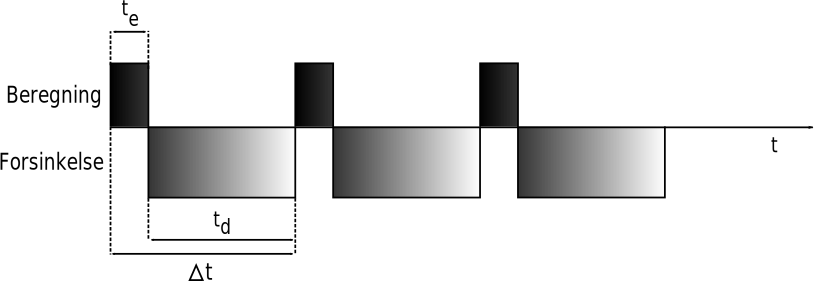
\includegraphics[width=.7\textwidth]{../brugere/kjaergaard/motorstyring-indlagt-forsinkelse}
  \caption{Motorstyring med indlagt forsinkelse.}
  \label{fig:motorstyring-indlagt-forsinkelse}
\end{figure}

Ved denne type motorstyring er tiden $t$ mellem
skridtene\fixme{fælles: andet ord?} givet ved
\begin{align}
  \Delta t &= t_e + t_d \nonumber \Rightarrow \\
  v &= \frac{\Delta x}{t_e + t_d}
\end{align}
hvor $t_d$ er den indlagte forsinkelse og $t_e$ er den tid det tager
at afvikle tidsberegningen. Da $t_e$ ikke kendes på
afviklingstidspunktet - og \textit{kan} variere fra afvikling til
afvikling afhængig af tallenes størrelse - er metoden upræcis ved høje
hastigheder. I figur\vref{fig:motorstyring-indlagt-forsinkelse-timing}
ses en situation, hvor størrelsen af $t_e$\fixme{kjærgaard: skriv
  afsnit færdigt, brug skitser fra egne notater}

\begin{figure}[htbp]
  \centering
  \vspace{3cm}
  \caption{Hastighed som funktion af forsinkelse for motorstyring med
    indlagt forsinkelse.}
  \label{fig:motorstyring-indlagt-forsinkelse-timing}
\end{figure}


\subsection{Motorstyring med afbrudt afvikling}

Alternativt kan motorerne times med afbrudt afvikling. Med en fast
fekvens tjekkes der, om det er tid til at flytte motorerne. Når der
ikke tjekkes om motorerne skal flyttes, beregnes det næste tidspunkt,
motorerne skal flyttes. Se
figur\vref{fig:motorstyring-afbrudt-afvikling}.

\begin{figure}[htbp]
  \centering
  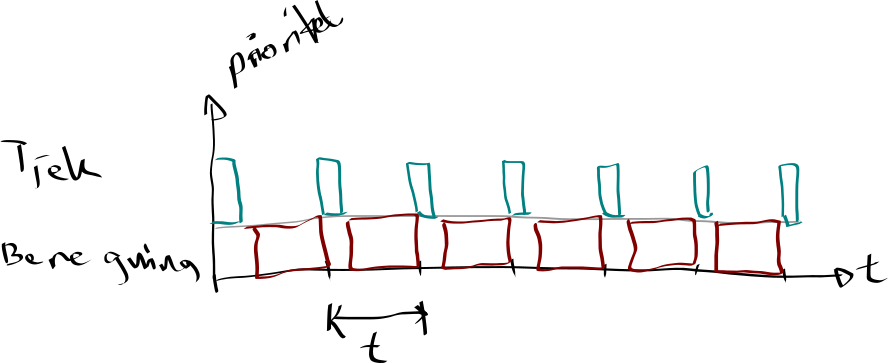
\includegraphics[width=.8\textwidth]{../brugere/kjaergaard/motorstyring-afbrudt-afvikling}
  \caption{Motorstyring med afbrudt afvikling.}
  \label{fig:motorstyring-afbrudt-afvikling}
\end{figure}

Den algoritme, der beregner hvilke tidspunkter, motorerne skal flyttes
på, afvikles hele tiden. Når det er tid til at tjekke, om vi har
overskredet et tidspunkt, afbrydes afviklingen af
beregningsalgoritmen, og tjekkeralgoritmen afvikles. Når
tjekkeralgoritmen\fixme{fælles: andet ord!} er afviklet, fortsættes
afviklingen af beregningen af tidspunkter.

Med denne metode kendes mindst mulige forsinkelse $t$, og vi har, hvad
vi efterspørger. Forskellige hastigheder opnås ved at udelade at
flytte motorerne på alle tidspunkter (se
figur\vref{fig:motorstyring-afbrudt-afvikling-hastighed}), og
præcisere styring af hastigheden opnås ved at afvikle
tjekkeralgoritmen med større frekvens. \fixme{kjærgaard: anden
  formulering}

\mnote{
  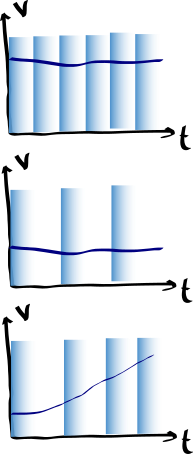
\includegraphics[width=\marginparwidth]{../brugere/kjaergaard/motorstyring-afbrudt-afvikling-hastighed}
  \captionof{figure}{Eksempel på høj hastighed, lav hastighed og
    acceleration ved motorstyring med afbrudt afvikling.}
  \label{fig:motorstyring-afbrudt-afvikling-hastighed}
}

Løsningen forudsætter, at
\begin{itemize}
\item dataene fra algoritmen, der beregner tidspunkter, kan opbevares
  i en kø,
\item der er data i køen, når tjekkeralgoritmen har brug for data at
  tjekke mod, og
\item beregningsalgoritmen kan afvikles så hurtigt, at der lægges data
  i køen hurtigere end tjekkeralgoritmen gennemgår dem.
\end{itemize}

I værste tilfælde skal behandlingsalgoritmen
\begin{itemize}
\item indlæse data fra datakilden,
\item fortolke dataene og
\item beregne tidspunktet
\end{itemize}

Med en taktfrekvens på 16 MHz

\subsection{Matematik -- motorkontrol}

Forholdet imellem tiden det tager at tegne linjen og tiden til et
punkt på linjen med $x$-koordinatet er lig forholdet imellem det givne
punkts x-koordinat og forskellen imellem start- og slutkoordinat $\Delta x$:

\begin{align}
\frac{t}{\Delta t} &= \frac{x}{\Delta x} \Rightarrow x(t) = \Delta x \times \frac{t}{\Delta t}
\end{align}

Den generelle formel for tiden $t$, det tager at tegne linjen, er lig:
\begin{align}
v &= \frac{L}{\Delta t} \Rightarrow \Delta t= \frac{L}{v}
\end{align}

Hvilket betyder, at vi kan kombinere (5.1) og (5.2):
\begin{align*}
\frac{t \times v}{L} &= \frac{x}{\Delta x}
\end{align*}

Ved isolering af tiden $t$ får vi at:
\begin{align}
t = \frac{x}{\Delta x} \times \frac{L}{v}
\end{align}

Længden af linjen $L$ er givet ud fra pythagoras læresætning:
\begin{align*}
L &= \sqrt{\Delta x^2+\Delta y^2}
\end{align*}

Forholdet imellem $x$ og $\Delta x$ kan beskrives som forholdet imellem step $n$ og total antal steps $\Delta n$:
\begin{align}
\frac{x}{\Delta x} = \frac{n}{\Delta n}
\end{align}

Indsættes dette i (5.3) får vi et udtryk for tiden $t$, som afhænger af step $n$:
\begin{align}
t &= \frac{n}{\Delta n} \times \frac{L}{v}
\end{align}

Step $n$ kan findes ved brug af følgende formel:
\begin{align}
n &= x \times \eta_x \qquad n \in{R}
\end{align}

Formlen fremkommer af vores definition på $\eta$, som er:
\begin{align*}
\eta_x = \frac{n}{x}
\end{align*}

Ud fra formlen fremgår det, at $\eta$ har enheden $\frac{steps}{mm}$.
Standardenheden, som er givet fra HPGL, er 0,025mm, altså en $\frac{1}{40}mm$

Figur\vref{fig:la-behandling} viser hvordan behandlingen foregår.
\begin{figure}[htbp]
  \centering
  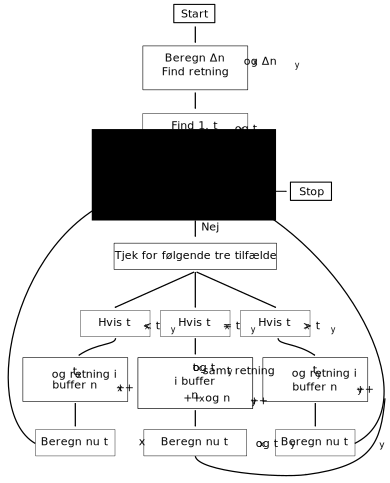
\includegraphics[width=.75\textwidth]{./img/la-behandling}
  \caption{Afviklingsdiagram over afvikling af LA-instruktionen.}
  \label{fig:la-behandling}
\end{figure}

\section{HPGL -- Hewlett-Packard Graphics Language}

Når man skal vælge, hvilket format man vil bruge, når man laver en
plotter, så er der en del ting at tage hensyn til. Der findes mange
forskellige standarder, som kan anvendes og en af disse standarder er
HPGL, som vi benytter os af.

Når man skal vælge, hvad man vil bruge, så er det vigtigt at se på
fordele og ulemper. Vi kunne i princippet godt udvikle vores eget
plotterformat, men dette vil både være meget tidskrævende, og
samtidigt vil det være svært at få implementeret, da vores format ikke
er en standard, og derfor er der ikke noget som direkte virker med
det. Derfor er HPGL velegnet i vores projekt, da det er mere
virkelighedsnært at benytte en standard, som allerede er konstrueret
som et plotterformat, samtidig med at det kan anvendes af forskellige
applikationer (andre CAD programmer). Der er heller ikke mange ulemper
tilknyttet til brugen af HPGL som plotterformat. Det vil dog tage lang
tid at implementere det hele, hvilket vi dog heller ikke gør. Vi
kommer f.eks. ikke til at benytte os af pin-skrift og en del andre
ting, men disse problemer er relativt lette at komme udenom.

Når man betragter HPGL som et plotterformat, så betyder det, at den
indeholder mange forskellige kommandoer med hver deres funktion. Det
kan tage lang tid at sætte sig ind i alle disse ting, men hvis man har
forståelse for, hvilke funktioner vi evt. kommer til at bruge i vores
projekt, vil det selvfølgelig lette indlæringsarbejdet en del.

Følgende er en tabel over vores overvejelser omkring fordele og
ulemper ved brugen af eget dataformat samt fordele og ulemper ved
brugen af HPGL:

%Eget dataformat
%Fordele	Ulemper
%•	Vi kan gøre det så simpelt som muligt, både til at læse og til at forstå (\fixme: uddyb)	•	Det vil nok afføde børnesygdomme
%•	Der findes ikke software, som kan håndtere vores dataformat


\fixme{Her indsættes tabel over fordele og ulemper ved eget
  dataformat. Denne tabel eksistere allerede}

Dette betyder, at der findes ingen software, der kan håndtere
formatet. Dette betyder at vi selv skal skrive den software, som er
uden for rammer af dette projekt. Derfor leder vi efter en
eksisterende standard.

\fixme{Her indsættes tabel over f og u ved HPGL}

Dette betyder, at HPGL er meget velegnet til brug i vores projekt, da
formatet er veldokumenteret, afprøvet og anvendt industrielt til
specielt plottere, hvilket vores eget selvfølgelig også ville være, og
der finde allerede software, som kan håndtere formatet til forskel fra
vores eget. Implementeringstiden vil dog være en del længere, da
niveauet er sat fra starten, hvilket medfører en del ubenyttede
funktioner.


\section{Koordinatsystem}

% Skriv om koordinatsystemet

Vi arbejder med skærmkoordinater (se
figur\vref{fig:skaermkoord}). HPGL (se
softwaredesignafsnit\fixme{kjærgaard:lav henvisning}) er formateret i
skærmkoordinater (og ikke Euklidiske koordinater?\fixme{tjek navn}),
og internt i softwaren (se igen
softwareafsnit\fixme{kjærgaard:henvisning}) kan en konvertering
springes over ved at bruge skærmkoordinater.

\snote{
  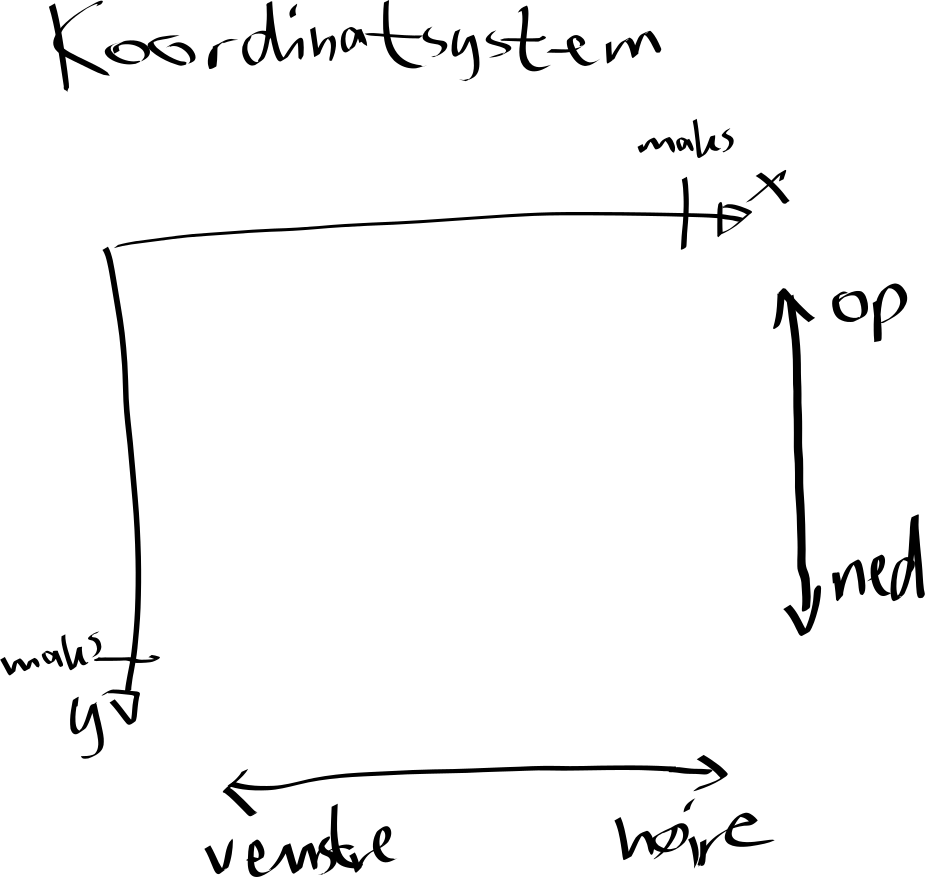
\includegraphics[width=\marginparwidth]{../brugere/kjaergaard/skaermkoordinater}
  \captionof{figure}{Skærm\-koor\-dinater. Der arbejdes med
    skærmkoordinater i plotteren.}
  \label{fig:skaermkoord}
}

\section{Valg af programmeringssprog}

Softwaren skrives i C og \Cpp.

C bruges i moduler, hvor sproget uden videre er tilstrækkeligt. Dette
vil typisk være lavniveaumoduler, og her er C fordelagtigt, fordi det
giver større kontrol.

\Cpp\ bruges i moduler, hvor det er fordelagtigt at bruge
\Cpp-speficikke elementer (f.eks. generisk programmering\fixme{note om
  dette?}). Moduler, der afhænger af moduler skrevet i \Cpp, vil
typisk også være skrevet i \Cpp.

Alle C-moduler er kompatible med \Cpp, og alle \Cpp-moduler er så vidt
muligt kompatible med C. Uønskede sideeffekter af \Cpp\ forsøges
undgået (\fixme{eksempler her!}). \Cpp\ bruges ikke objektorienteret.



%%% Local Variables: 
%%% mode: latex
%%% TeX-master: "../master"
%%% End: